\section{Software Update Platform}

Software Update Platform is responsible for performing updates on multiple devices and monitoring
installed applications. Developers prepare \emph{.deb} packages with applications and add them to
repository. When connection with device is established and information about update is written in
database, platform will perform software update on that device.


\subsection{Architecture}

Software Update Platform consists of two main parts:
\begin{itemize}
  \item client application installed on mobile device,
  \item server.
\end{itemize}

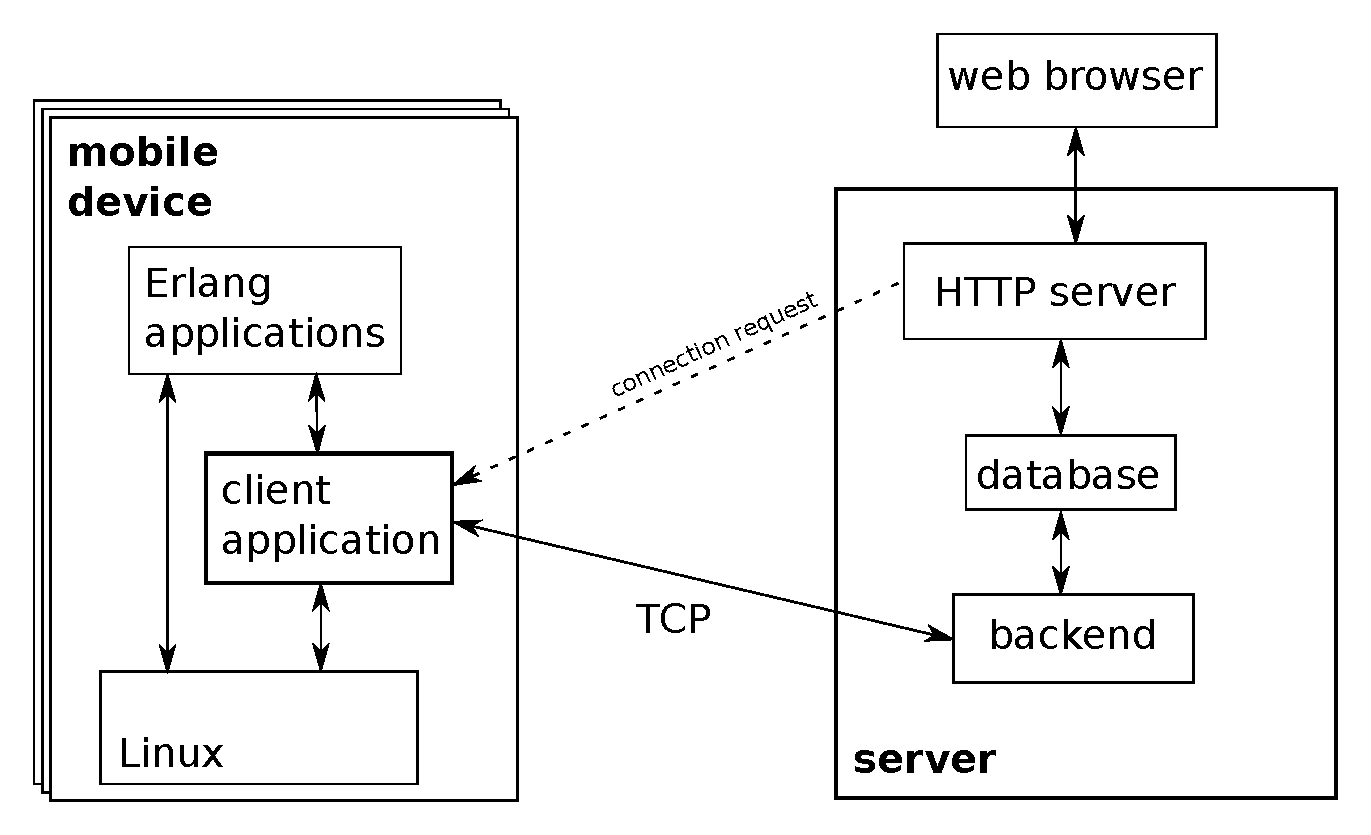
\includegraphics[width=\textwidth]{graphics/architecture.pdf}


\subsubsection*{Client application}

We assume that client application is running on Erlang VM installed on some Linux distribution and
\emph{apt} is available. Client application connects with server and perform given operations.


\subsubsection*{Server}

Server consists of 3 components:
\begin{itemize}
  \item HTTP server
  \item database
  \item backend
\end{itemize}


\subsubsection*{HTTP server}

Mochiweb -- our web server of choice is responsible for following tasks. It manages user interaction
through web interface (serves content, performs user requests) and it is repository for \emph{.deb}
packages.


\subsubsection*{Database}

Mnesia database stores information about:
\begin{itemize}
  \item device and installed applications on it,
  \item jobs (e.g.\ update) for device.
\end{itemize}

\noindent Database is connector beetwen web interface and backend. It stores user requests -- jobs to perform
on device.


\subsubsection*{Backend}

Backend is the core of platform. It is Erlang application responsible for whole automatic device
management. Every new device in platform connected with backend is stored in database.
From now on backend can monitor state of that device and performs operations on it.

\subsubsection{Device-server session}
\subsubsection{On-device upgrade logic}

\subsection{Functionality}

\begin{itemize}
	\item General description of the application: Web interface, technology
    \item Development model for application, debian packaging utilities
    \item Direct usage of package manager on remote devices 
\end{itemize}

gui: 1 or 2 images 

